\documentclass[english,a4paper,11pt,oneside]{article}
\usepackage[utf8]{inputenc}
\usepackage{hyperref}
\usepackage{babel}
\usepackage{amsmath}
\usepackage{amsfonts}
\usepackage{amssymb}
\usepackage{graphicx}
\usepackage{xcolor}
\usepackage[rightlabels]{titletoc}
\usepackage{pdfpages}
\usepackage{grffile}
\usepackage[export]{adjustbox}
\usepackage{listings}
\usepackage{datetime}  
\usepackage{sectsty}
\usepackage{python}
\NeedsTeXFormat{LaTeX2e}
\ProvidesPackage{pythonhighlight}[2011/09/19 python code highlighting; provided by Olivier Verdier <olivier.verdier@gmail.com>]


\RequirePackage{listings}
\RequirePackage{xcolor}

\renewcommand*{\lstlistlistingname}{Code Listings}
\renewcommand*{\lstlistingname}{Code Listing}
\definecolor{gray}{gray}{0.5}
\colorlet{commentcolour}{green!50!black}

\colorlet{stringcolour}{red!60!black}
\colorlet{keywordcolour}{magenta!90!black}
\colorlet{exceptioncolour}{yellow!50!red}
\colorlet{commandcolour}{blue!60!black}
\colorlet{numpycolour}{blue!60!green}
\colorlet{literatecolour}{magenta!90!black}	
\colorlet{promptcolour}{green!50!black}
\colorlet{specmethodcolour}{violet}

\newcommand*{\framemargin}{3ex}

\newcommand*{\literatecolour}{\textcolor{literatecolour}}

\newcommand*{\pythonprompt}{\textcolor{promptcolour}{{>}{>}{>}}}

\lstdefinestyle{mypython}{
	%\lstset{
	%keepspaces=true,
	language=python,
	showtabs=true,
	tab=,
	tabsize=2,
	basicstyle=\ttfamily\footnotesize,%\setstretch{.5},
	stringstyle=\color{stringcolour},
	showstringspaces=false,
	alsoletter={1234567890},
	otherkeywords={\%, \}, \{, \&, \|},
	keywordstyle=\color{keywordcolour}\bfseries,
	emph={and,break,class,continue,def,yield,del,elif ,else,%
		except,exec,finally,for,from,global,if,import,in,%
		lambda,not,or,pass,print,raise,return,try,while,assert,with},
	emphstyle=\color{blue}\bfseries,
	emph={[2]True, False, None},
	emphstyle=[2]\color{keywordcolour},
	emph={[3]object,type,isinstance,copy,deepcopy,zip,enumerate,reversed,list,set,len,dict,tuple,xrange,append,execfile,real,imag,reduce,str,repr},
	emphstyle=[3]\color{commandcolour},
	emph={Exception,NameError,IndexError,SyntaxError,TypeError,ValueError,OverflowError,ZeroDivisionError},
	emphstyle=\color{exceptioncolour}\bfseries,
	%upquote=true,
	morecomment=[s]{"""}{"""},
	commentstyle=\color{commentcolour}\slshape,
	%emph={[4]1, 2, 3, 4, 5, 6, 7, 8, 9, 0},
	emph={[4]ode, fsolve, sqrt, exp, sin, cos,arctan, arctan2, arccos, pi,  array, norm, solve, dot, arange, isscalar, max, sum, flatten, shape, reshape, find, any, all, abs, plot, linspace, legend, quad, polyval,polyfit, hstack, concatenate,vstack,column_stack,empty,zeros,ones,rand,vander,grid,pcolor,eig,eigs,eigvals,svd,qr,tan,det,logspace,roll,min,mean,cumsum,cumprod,diff,vectorize,lstsq,cla,eye,xlabel,ylabel,squeeze},
	emphstyle=[4]\color{numpycolour},
	emph={[5]__init__,__add__,__mul__,__div__,__sub__,__call__,__getitem__,__setitem__,__eq__,__ne__,__nonzero__,__rmul__,__radd__,__repr__,__str__,__get__,__truediv__,__pow__,__name__,__future__,__all__},
	emphstyle=[5]\color{specmethodcolour},
	emph={[6]assert,yield},
	emphstyle=[6]\color{keywordcolour}\bfseries,
	emph={[7]range},
	emphstyle={[7]\color{keywordcolour}\bfseries},
	% emph={[7]self},
	% emphstyle=[7]\bfseries,
	literate=*%
	{:}{{\literatecolour:}}{1}%
	{=}{{\literatecolour=}}{1}%
	{-}{{\literatecolour-}}{1}%
	{+}{{\literatecolour+}}{1}%
	{*}{{\literatecolour*}}{1}%
	{**}{{\literatecolour{**}}}2%
	{/}{{\literatecolour/}}{1}%
	{//}{{\literatecolour{//}}}2%
	{!}{{\literatecolour!}}{1}%
	%{(}{{\literatecolour(}}{1}%
	%{)}{{\literatecolour)}}{1}%
	{[}{{\literatecolour[}}{1}%
	{]}{{\literatecolour]}}{1}%
	{<}{{\literatecolour<}}{1}%
	{>}{{\literatecolour>}}{1}%
	{>>>}{\pythonprompt}{3}%
	,%
	%aboveskip=.5ex,
	frame=trbl,
	%frameround=tttt,
	%framesep=.3ex,
	rulecolor=\color{black!40},
	%framexleftmargin=\framemargin,
	%framextopmargin=.1ex,
	%framexbottommargin=.1ex,
	%framexrightmargin=\framemargin,
	%framexleftmargin=1mm, framextopmargin=1mm, frame=shadowbox, rulesepcolor=\color{blue},#1
	%frame=tb,
	backgroundcolor=\color{white},
	breakindent=.5\textwidth,frame=single,breaklines=true%
	%}
}

\newcommand*{\inputpython}[3]{\lstinputlisting[firstline=#2,lastline=#3,firstnumber=#2,frame=single,breakindent=.5\textwidth,frame=single,breaklines=true,style=mypython]{#1}}

\lstnewenvironment{pythonn}[1][]{\lstset{style=mypython}}{}

\lstdefinestyle{mypythoninline}{
	style=mypython,%
	basicstyle=\ttfamily,%
	keywordstyle=\color{keywordcolour},%
	emphstyle={[7]\color{keywordcolour}},%
	emphstyle=\color{exceptioncolour},%
	literate=*%
	{:}{{\literatecolour:}}{2}%
	{=}{{\literatecolour=}}{2}%
	{-}{{\literatecolour-}}{2}%
	{+}{{\literatecolour+}}{2}%
	{*}{{\literatecolour*}}2%
	{**}{{\literatecolour{**}}}3%
	{/}{{\literatecolour/}}{2}%
	{//}{{\literatecolour{//}}}{2}%
	{!}{{\literatecolour!}}{2}%
	%{(}{{\literatecolour(}}{2}%
	%{)}{{\literatecolour)}}{2}%
	{[}{{\literatecolour[}}{2}%
	{]}{{\literatecolour]}}{2}%
	{<}{{\literatecolour<}}{2}%
	{<=}{{\literatecolour{<=}}}3%
	{>}{{\literatecolour>}}{2}%
	{>=}{{\literatecolour{>=}}}3%
	{==}{{\literatecolour{==}}}3%
	{!=}{{\literatecolour{!=}}}3%
	{+=}{{\literatecolour{+=}}}3%
	{-=}{{\literatecolour{-=}}}3%
	{*=}{{\literatecolour{*=}}}3%
	{/=}{{\literatecolour{/=}}}3%
	%% emphstyle=\color{blue},%
}

\newcommand*{\pyth}{\lstinline[style=mypythoninline]}

\renewcommand{\contentsname}{Sommaire}
\renewcommand{\thesection}{\Roman{section}} 
%\renewcommand{\thesubsection}{\Roman{subsection}}
\definecolor{armygreen}{rgb}{0.05, 0.5, 0.06}
%-% Problèmes résumé
%-% Trop de retour à la ligne
%-% Suites des phrases
%-% Pas bsn de mettre en gras, italique les mots cléfs. Par contre mettre en caractères spéciales les commandes + code

\titlecontents{subsection}% <section>
[2.35em]% <left>
{\small\contentsmargin{1.5em}}% <above-code>
{\thecontentslabel.\hspace{3pt}}% <numbered-entry-format>; you could also use {\thecontentslabel. } to show the numbers
{}% <numberless-entry-format>
{\enspace\titlerule*[0.5pc]{.}~\contentspage}% <filler-page-format>

\usepackage{float}
\usepackage{listings}
%\lstinputlisting[language=Python, firstline=0, lastline=15]{main.py}
\definecolor{googleblue}{HTML}{0F9D58}
\definecolor{googlegreen}{HTML}{4285F4}
\definecolor{googlered}{HTML}{DB4437}
\definecolor{googleyellow}{HTML}{F4B400}

\sectionfont{\color{googlered} \normalfont} % sets colour of sections
\subsectionfont{\color{googlegreen} \normalfont}  % sets colour of sections
\subsubsectionfont{\color{googleblue} \normalfont}  % sets colour of sections

\author{\color{blue} \raggedright GHOUIBI GHASSEN}
\title{\color{red} \normalfont\huge Fiche de lecture pour }
\begin{document}

	 \begin{titlepage}
		\centering 
		%
		\vspace{1cm}
		
		\vspace{0.5cm}
		{\huge\bfseries 20 Newsgroup \par}
		\vspace{0.5cm}
		\vfill
		{\Large\itshape Text Mining  \par}
		\vfill
		% Bottom of the page
		{\large Auteur  \par
			KHEMIRI Rami \par
			GHOUIBI Ghassen\textsc{}\par}
		\vspace{1cm}
		{\large Encadrée \par
			Mr. Nistor Grozavu \textsc{}\par
			
		}
	\end{titlepage}
	\tableofcontents
	\newpage
	\section{Introduction}{
		Ce rapport correspond au projet '20newsgroup', qui composé d'un ensemble de données texte on va explorer ces données en utilisant l'apprentissage automatique et en tirer des informations.\\
		Les sections dans ce rapport seront de cet ordre :
		\begin{itemize}
			\item Text Processing and Transformation
			\item Analysis of the dataset
			\item Machine Learning
			\item Visualization
			\item Theoretical details
			\item Conclusion
		\end{itemize}
		Notre choix se porte sur le language Python pour la réalisation de ce projet.
		
	}
	
	\section{Text Processing and Transformation}{
		\subsection{Extracting features from text files}{
			Pour transformer le texte en vecteurs on aura besoin de étape pour y arrivé, en utilisant \texttt{Bag of words} et \texttt{Tokenizing text}.\\
			Dans cette section on à suivi le tutoriel \href{https://scikit-learn.org/stable/tutorial/text_analytics/working_with_text_data.html#tutorial-setup}{suivant}.
			\subsubsection{Bags of words}{
				Bag of words, est une représentation simplificatrice utilisé dans le traitement du langage naturel et la recherche d'informations.\\
				Dans ce modèle un texte est représenté comme le sac de ses mots sans tenir compte de la grammaire et même l'ordre des mots mais en gardant la multiplicité.\\
				On va tout simplement attribuer un entier à chaque mot dans un texte on prend un exemple\footnote{Cette exemple est pris de wikipedia \\ \url{https://en.wikipedia.org/wiki/Bag-of-words_model}}: \\
				\itshape{John likes to watch movies. Mary likes movies too.}\\
				\itshape{BoW1 = \{"John":1,"likes":2,"to":1,"watch":1,"movies":2,"Mary":1,"too":1\};}
			}
			\newpage
			\subsubsection{Tokenizing text}{
				Dans cette partie on va essayer de \texttt{tokeniser} le texte, c'est le processus de conversion d'une séquence de caractères en une séquence de jetons (chaînes avec une signification assignée et don identifiée).\\
				Notre but principale c'est transformer ce texte en vecteur, le prétraitement du texte, tokenisation et filtrage des mots sont inclut dans \texttt{CountVectorizer}.\\
				\begin{pythonn}
from sklearn.feature_extraction.text import CountVectorizer
count_vect = CountVectorizer()
X_train_counts = count_vect.fit_transform(twenty_train.data)
				\end{pythonn}
			
				\texttt{CountVectorizer} prend en charge le nombre de N-grammes de mots ou de caractères consécutifs. Une fois installé, le vectoriseur a construit un dictionnaire d'indices.\\
				En effet, on va esssaye d'approndir la variable \texttt{X\_train\_counts} est une \texttt{sparse} matrice qu'on va utiliser parce qu'elle supporte l'addition, multiplication, divsion et matrix power.\\
				Avec une dimension égale à 2 notre matrice est composé d'un tuple et un indice(nombre d'occurences) d'où on voulait savoir leur attribut et ce qu'on peut extraire comme informations de cette matrice voici les attributs:
				\begin{itemize}
					\item dtype : type de matrice
					\item shape : shape de matrice
					\item ndim  : dimension de matrice 
					\item nnz   : nombre de valeur stockée (incluant les zéro)
				\end{itemize}
				
			}
		}
		\subsection{From occurrences to frequencies}{
		 Extraire le nombre d'occurrences est un bon début mais il y a un problème pour les textes plus longs auront des moyennes plus élevées ques les documents les plus courts, même s'ils parlent du même sujets.\\
		 Pour éviter ces divergences il suffit de diviser le nombre d'occurences de chaque mot dans un texte par le nombre total de mots dans le texte, ces nouvelles \texttt{features} sont appelées tf \texttt{Term Frequency}.\\
		 Une autre opération est recommander c'est réduire l'échelle des poids pour les mots qui apparaissent dans des nombreux textes du corpus et sont donc moins informatifs que ceux qui n'apparaissent que dans une petite partie du corpus.\\
		 \newpage
		 \begin{pythonn}
from sklearn.feature_extraction.text import TfidfTransformer
tfidf_transformer = TfidfTransformer()
X_train_tfidf = tfidf_transformer.fit_transform(X_train_counts)
		 \end{pythonn}
		 Dans le code ci-dessus, nous utilisons la méthode \texttt{fit\_tranform} pour transformer notre matrice de comptage en une représentation \texttt{tf-idf} en ignorant le traitement redondant.
		 En accédant à la variable \texttt{X\_train\_tfidf.data} on remarque notre matrice est normaliser maintenant au plutôt représente en \texttt{tfidf}.\\
		 
		 TF-IDF\footnote{Cette définition est prise à partir de wikipedia \url{https://fr.wikipedia.org/wiki/TF-IDF}} est une méthode de pondération souvent utilisée en recherche d'information et fouilles de textes.Cette mesure statistique permet d'évaluer l'importance d'un terme contenu dans un document, relativement à une collection ou un corpus.\\
		 Le poids augmente proportionnellement au nombre d'occurrences du mot dans le document. Il varie également en fonction de la fréquence du mot dans le corpus.\\
		 Des variantes de la formule originale sont souvent utilisées dans des moteurs de recherche pour apprécier la pertinence d'un document en fonction des critères de recherche de l'utilisateur.
		 
		}
	}
	\section{Analysis of the dataset}{
		Dans cette section on va essayer d'analyser notre dataset, nous allons commencer par extraire quelques informations statistiques, vérifier les valeurs manquantes, les outliers, la correlation entre les variables et finir par présenté le but de cette analyse.
		\subsection{Dataset Shape}{
			Avant de regarder dans notre dataset et visualiser sa forme il faut comprendre notre data, dans le cas on a choisi de créer un classe Dataset qui va nous permettre de faire des opérations dessus sans polluer notre code.\\
			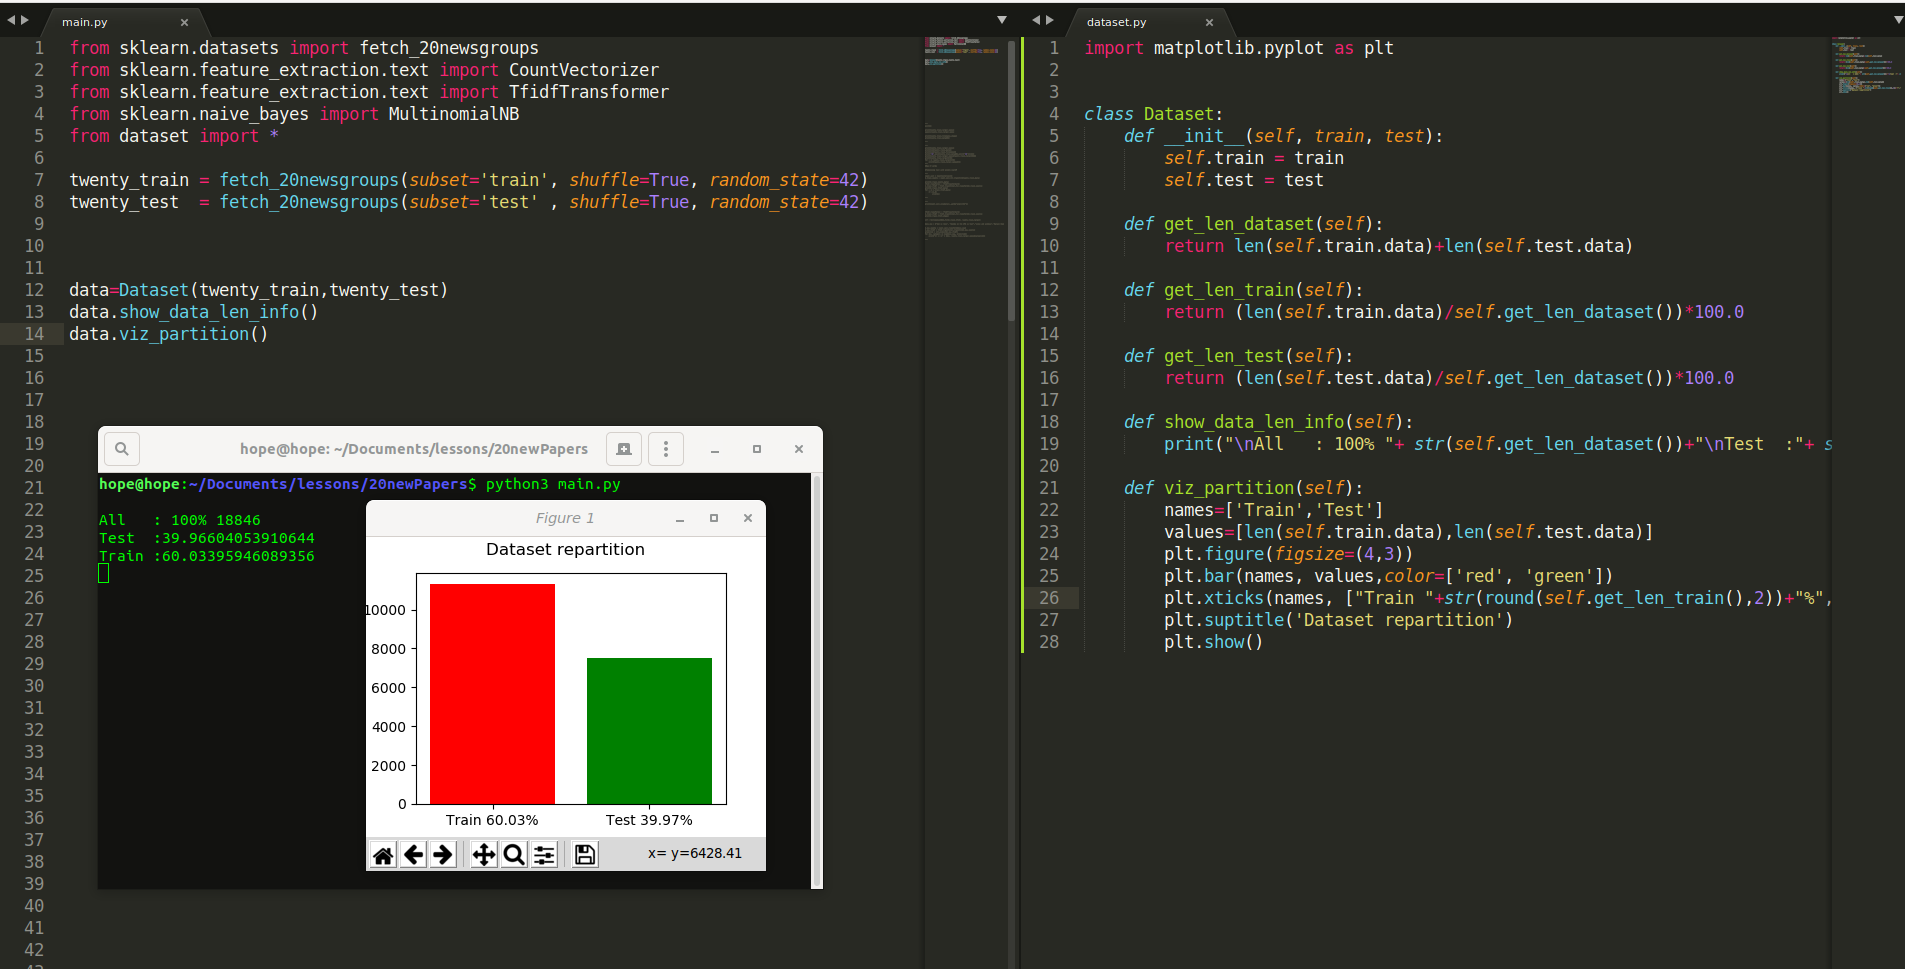
\includegraphics[width=350pt]{1}
			
			On va continuer sur la même classe concernant notre analyse du dataset, en effet avec un simpe appel a une méthode on obtient le shape de notre dataset de trainning.\\
		}
		\subsection{Outliers}{
			Un outlier peut être :
			\begin{itemize}
			\item une valeur {\itshape aberrante}: c'est une valeur qui est manifestement fausse
			\item une valeur {\itshape atypique }: c'est une valeur qui "sort du lot", mais pas forcément fausse.
			\end{itemize}
			Dans cette partie on choisi de faire un fonction qui va nous permettre de détécter les outliers dans notre dataset on a réussi à déduire quelque mots qui seront commun dans notre dataset on trouve quasiement toujours le nombre de lignes ainsi le sujet du mail passé par l'organization et le sujet d'où notre fonction était mise en place pour pouvoir savoir le nombre des valeurs manquante et leur impacte sur notre dataset si jamais le nombre est trés grand il faudra trouvé une solution voici un exemple du résultat obtenu:\\
			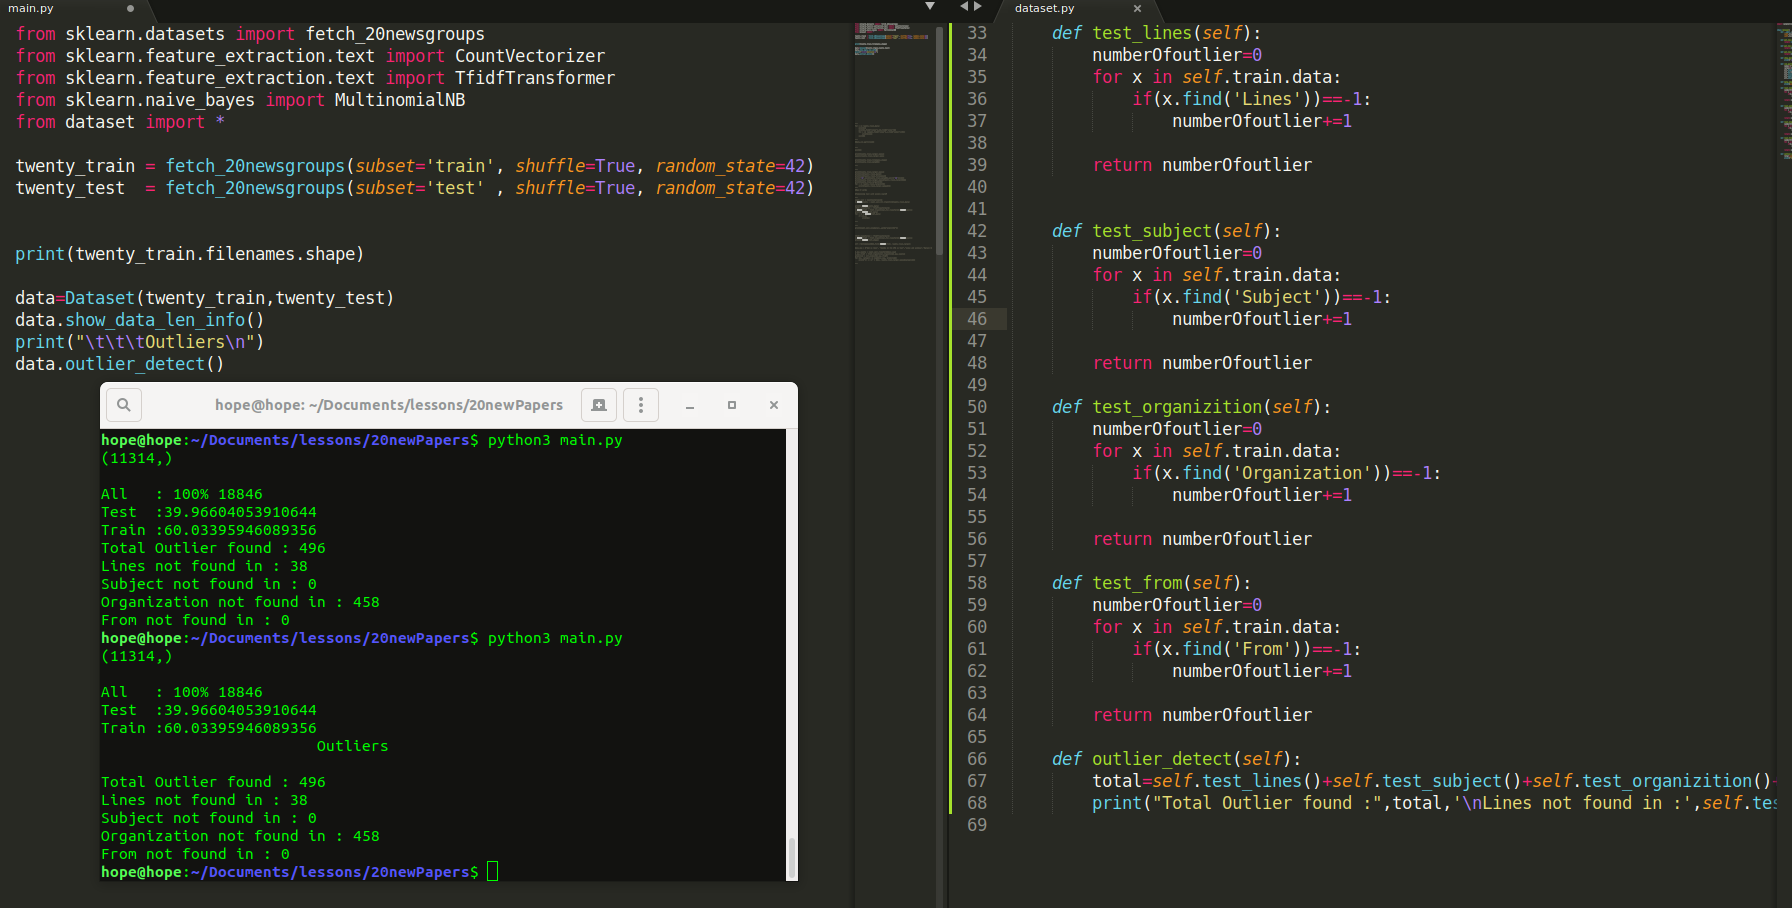
\includegraphics[width=350pt]{2}
			
			On remarque dans la figure ci-dessus que la totalité de nos outliers sont 496 contre 11314 initial qui ne réprésente que 4.38\% de notre dataset  
			
		}
		\subsection{Correlation between variables}{
			Les variables d'une dataset peuvent être liées pour plusieurs raisons par exemple une variable peut dépendre d'une autre ou il existe une association même deux variables dépend d'un troisème inconnu.\\
			Une correlation positive c'est à dire les deux variables bouge dans la même direction, quand c'est négative c'est à dire dans la direction inverse ou peut aussi être neutre dans ce cas il y a de relation entre ces deux variables.\\
			\begin{pythonn}
from sklearn.metrics import matthews\_corrcoef
def correlation(self,v1,v2):
	print(matthews_corrcoef(v1,v2))
			\end{pythonn}
			On a trouve une correlation positive entre le texte et la catégorie.
			
		}
	
			
	}
	\section{Machine learning}{
		Dans cette partie on va étudier de plus prés quelques modèles de machine learning, mais avant de tester nos modèles il faudra détaillé notre but.\\
		En effet on remarque bien que notre dataset est composé de texte, et chaque texte est représenté par un sujets dans notre cas c'est des catégories:\\
		\begin{pythonn}
def get_categories(self):
	print(self.train.target_names)
		\end{pythonn}
		\newpage
		On remarque qu'on 20 catégories, on va essayer d'appliquer des modèles sur le texte sans prendre en compte quelque paramètres (en eliminant quelques informations) pour pouvoir prédire notre catégorie donc notre target sera le sujet du texte.\\
		On va voir plus en détails avec les modèles choisi qu'on aura la chance de pouvoir visualiser quelques résultat.\\
		
		\subsection{Regression Line}{
			On parle de modèles linéaire ou modèle de régression linéaire quand on cherche à établir une relation variable dite expliquée et une ou plusieurs varabiles dites explicatives.\\
			Le modèle\footnote{prise de wikipedia \url{https://fr.wikipedia.org/wiki/R\%C3\%A9gression\_lin\%C3\%A9aire} } de régression linéaire est souvent estimé par la méthode des moindres carrés mais il existe aussi de nombreuses autres méthodes pour estimer ce modèle. On peut par exemple estimer le modèle par maximum de vraisemblance ou encore par inférence bayésienne.\\
			Dans cette sous section on va essayer de prédire quelques variables, on a choisi de travailler sur la target 'Lines' qui est représente dans nos outliers au par avant.\\
			
		}
		\subsection{K-NN}{
			Notre choix se porte sur K-NN, la méthode des k plus proches voisins est une méthode d'apprentissage supervisé.\\
			Pour\footnote{Prise de wikipedia \url{https://fr.wikipedia.org/wiki/M\%C3\%A9thode_des_k_plus_proches_voisins}} estimer la sortie associée à une nouvelle entrée x, la méthode des k plus proches voisins consiste à prendre en compte (de façon identique) les k échantillons d'apprentissage dont l’entrée est la plus proche de la nouvelle entrée x, selon une distance à définir.\\
			\newpage
			\begin{pythonn}
def knn(self,test,data,target,categories):
	print("-----------------KNN--------------------------------")
	count_vect = CountVectorizer()
	X_train_counts = count_vect.fit_transform(data)
	tfidf_transformer = TfidfTransformer()
	X_train_tfidf = tfidf_transformer.fit_transform(X_train_counts)
	
	clf = KNeighborsClassifier(n_neighbors=7).fit(X_train_tfidf, target)
	X_new_counts = count_vect.transform(test)
	X_new_tfidf = tfidf_transformer.transform(X_new_counts)
	predicted = clf.predict(X_new_tfidf)
	print("Predicted categories is :",categories[predicted[0]],"with score  \%",round(clf.score(X_train_tfidf, target)*100.0,2))
				
			\end{pythonn}
			
			Une représentation graphique sera attribuer dans la section Visualization.
		}
		\subsection{Naive base}{
			notre choix se porte sur Naive base vu que ce dernier est présent dans notre tutoriel, c'est un type de classification probabilist basé sur le théorème de Bayes avec une forte indépendance des phypothèses.\\
			\begin{equation}
				P(A|B)=\frac{P(B|A) . P(A)}{P(B)}
			\end{equation}
			où P(A/B)  désigne la probabilité conditionnelle de A sachant B.
		\newpage
		\begin{pythonn}
def naive_bayes(self,test,data,target,categories):
			
	print("-----------------Naive-Bayes------------------------")
	count_vect = CountVectorizer()
	X_train_counts = count_vect.fit_transform(data)
	tfidf_transformer = TfidfTransformer()
	X_train_tfidf = tfidf_transformer.fit_transform(X_train_counts)
	
	clf = MultinomialNB().fit(X_train_tfidf, target)
	X_new_counts = count_vect.transform(test)
	X_new_tfidf = tfidf_transformer.transform(X_new_counts)
	predicted = clf.predict(X_new_tfidf)
	print("Predicted categories is :",categories[predicted[0]],"with score  \%",round(clf.score(X_train_tfidf, target)*100.0,2))

		\end{pythonn}
	
		Une représentation graphique sera attribuer dans la section Visualization.	
	}
	
	\subsection{Linear SVC}{
	SVM\footnote{prise de wikipedia \url{https://fr.wikipedia.org/wiki/Machine\_\%C3\%A0_vecteurs_de_support}} sont un ensemble de technique d'apprentissage supervisé destinées à résoudre des problèmes de discrimination et de régression.\\
	Les SVM sont une généralisation des classifieurs linéaires.\\
	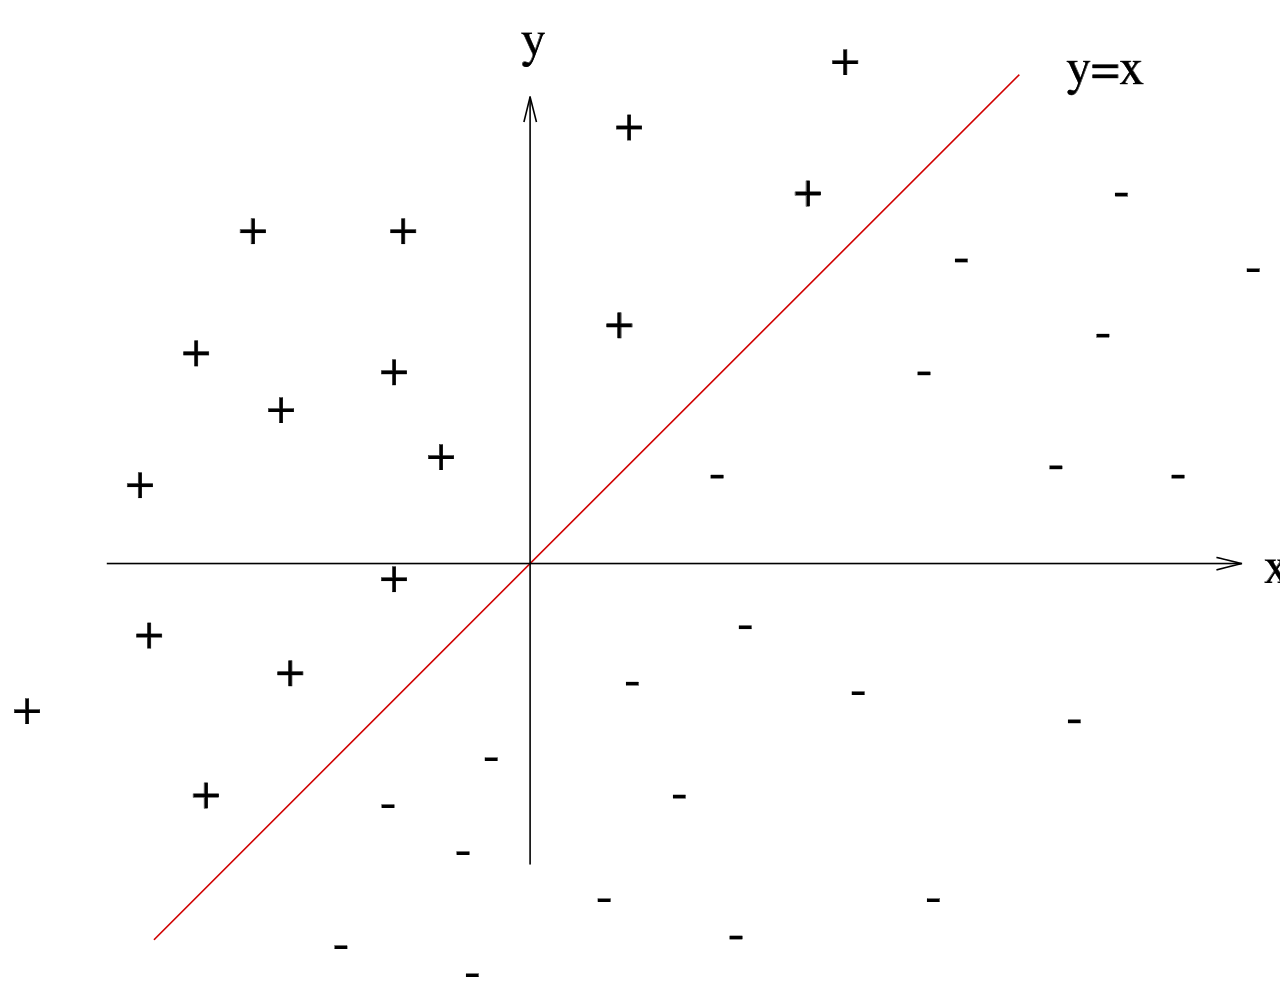
\includegraphics[width=300pt]{svm}\\
	Exemple d'un problème de discrimination à deux classes, avec une séparatrice linéaire : la droite d'équation y = x. Le problème est linéairement séparable.
	
		
	}
	\subsection{Analyze result}{
		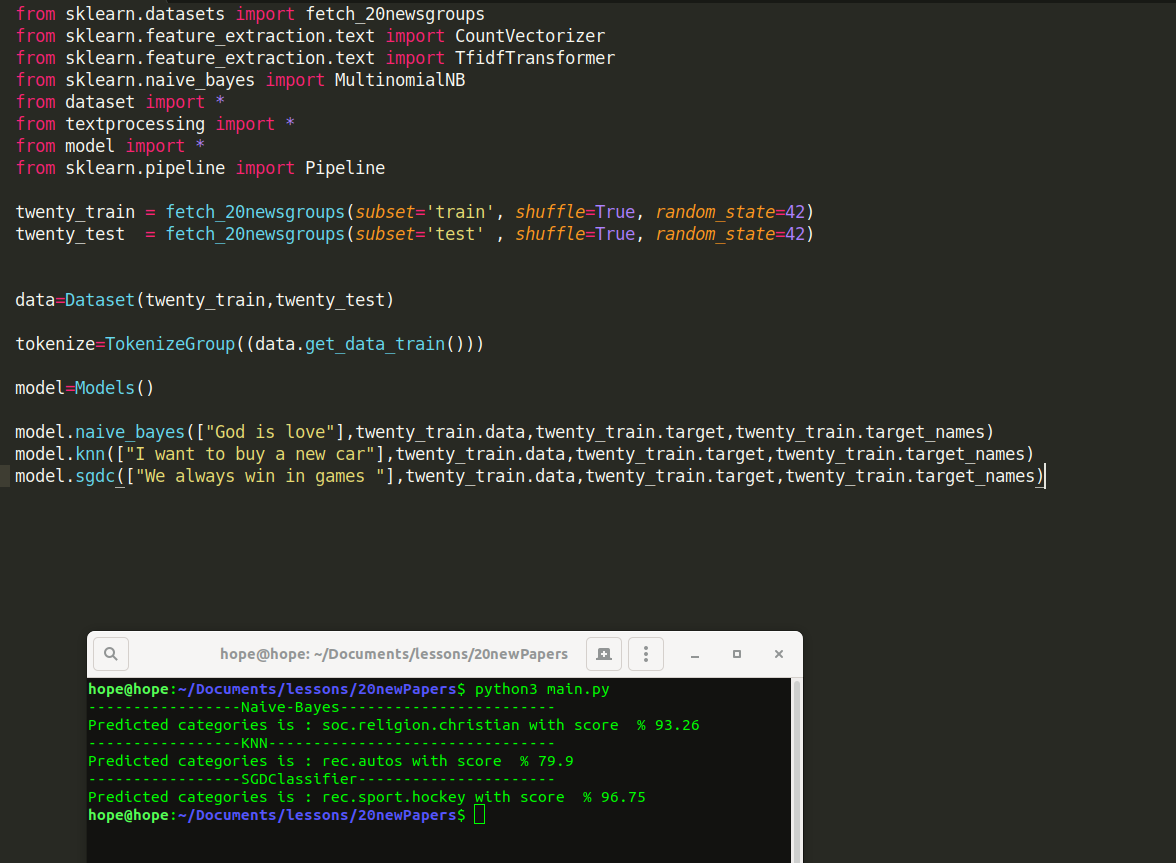
\includegraphics[width=350pt]{3}
		
		La figure ci-dessus montre l'utilisation des modèles sur une phrase pour prédire la catégories avec un score pour chaque modèle.

	}
	}

	\section{Visualization}{
		Dans cette partie on a choisi de visualiser les résultats de KMeans, tout d'abord il faudrat faire quelques manipulation sur notre dataset, on commence par choisir 3 catégories :\\
		\begin{itemize}
			\item 'comp.sys.mac.hardware'
			\item 'rec.autos'
			\item 'soc.religion.christian'
		\end{itemize}
		Pour des raisons de ressources on va prendre 200 échantillons, le nombre de nos clusters sera trois vu qu'on a trois catégories, ensuite on va transformer ce texte en \texttt{tfidf} on apliquer notre algorithme Kmeans voici les paramètres chosisi:\\
		\begin{pythonn}
			clustering_model = KMeans(
			n_clusters=3,
			max_iter=500,
			precompute_distances="auto",
			n_jobs=-1
			)
		\end{pythonn}
		
		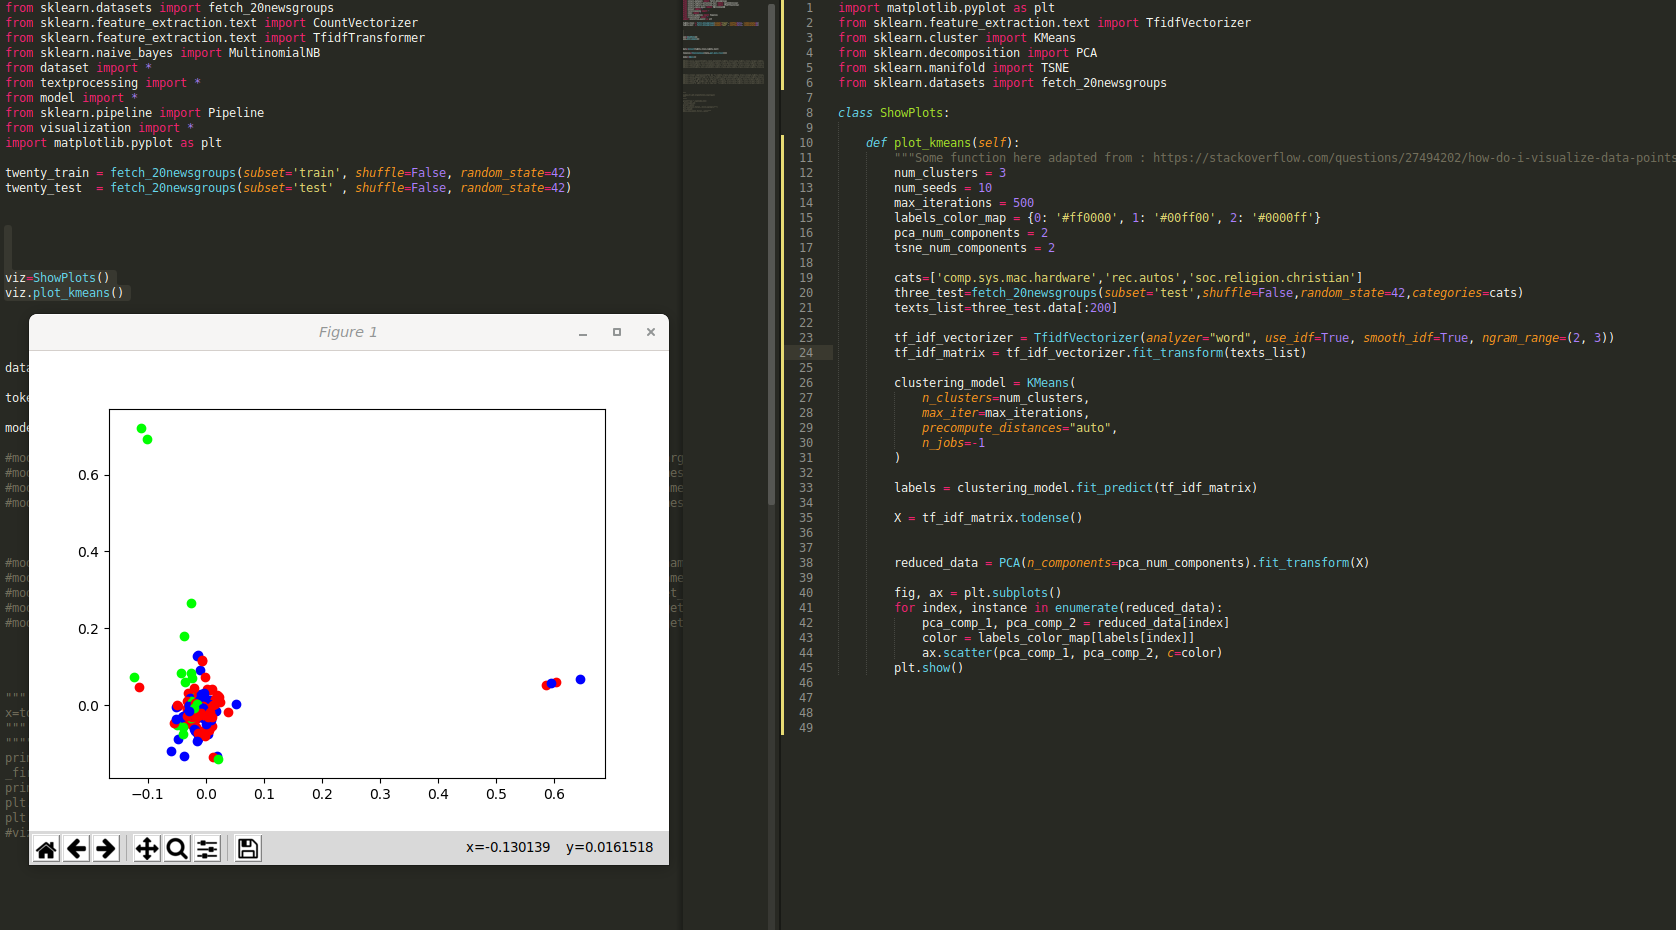
\includegraphics[width=350pt]{9}
		
		Voici un visualisation du résultat obtenu.
		
		
	}

	\section{Theoretical details}{
		Dans cette partie on va mettre en compétition nos modèles utilisés durant ce rapport ou inclus dans le code.\\
		Tout d'abord on va découper notre data pour travailler sur une partie on va prendre 100 texte pour tester et voici le résultat obtenu :\\
		\begin{tabular}{ |l|c| r|}
			\hline
			Model &  Score \\ \hline
			Naive Bayes & 0.932 \\ \hline
			K-NN & 0.799 \\ \hline
			SGDClassifier & 0.967 \\ \hline
			SVM 		&  0.999 \\ \hline
		\end{tabular}
		
		On remarque dans le tableau ci-dessus que notre modèle SVM obtient le meilleur score du coup on va regarder de plus prêt les paramètres et sa particularité.\\
		\newpage
		\begin{pythonn}
			clf = LinearSVC(C=1,
			  class_weight=None,
			  dual=True,
			  fit_intercept=True,
			  intercept_scaling=1,
			  loss='squared_hinge',
			  max_iter=1000,
			  multi_class='ovr',
			  penalty='l2',
			  random_state=None,
			  tol=0.01,
			  verbose=0)
		\end{pythonn}
		\begin{itemize}
			\item C: Paramètre de régularisation. La force de la régularisation est inversement proportionnelle à C. Doit être strictement positive.
			\item class\_weight :
			\item dual :Contrôle la génération de nombres pseudo aléatoires pour mélanger les données à double coordonnée.
			\item fit\_intercept : Indique s'il faut calculer l'ordonnée à l'origine pour ce modèle.
			\item loss : Spécifie la fonction de perte. «hinge» est la perte SVM standard (utilisée par exemple par la classe SVC) tandis que «squared\_hinge» est le carré de la perte.
			\item max\_iter : The maximum number of iterations to be run.
			\item multi\_class : Détermine la stratégie multi-classes si y contient plus de deux classes. "ovr" forme n\_classes classificateurs, tandis que "crammer\_singer" optimise un objectif commun sur toutes les classes.
			\item penalty : Spécifie la norme utilisée dans la pénalisation. La pénalité «l2» est la norme utilisée dans SVC. Le «l1» conduit à des vecteurs coef\_ .
			\item random\_state : Contrôle la génération de nombres pseudo aléatoires pour mélanger les données.
			\item tol : Tolérance pour les critères d'arrêt.
			\item verbose : Activer la sortie détaillée.
			
		\end{itemize}
		
	}



  


\end{document} 